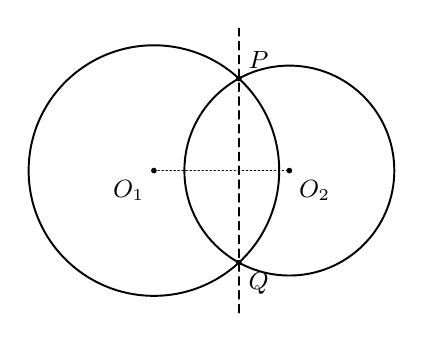
\begin{tikzpicture}[scale=0.86, line cap=round, line join=round, every node/.style={font=\small}]
    \coordinate (O1) at (-1,0);
    \coordinate (O2) at (1,0);
    \coordinate (P) at ({51/200},{sqrt(1.847475)});
    \coordinate (Q) at ({51/200},{-sqrt(1.847475)});
    \draw[line width=0.70pt] (O1) circle (1.85);
    \draw[line width=0.70pt] (O2) circle (1.55);
    \draw[densely dashed,line width=0.5pt] ({51/200},-2.1)--({51/200},2.1);
    \draw[densely dotted,line width=0.45pt] (O1)--(O2);
    \foreach \X in {O1,O2,P,Q} {\fill (\X) circle (1.2pt);}
    \node[below left] at (O1) {$O_1$};
    \node[below right] at (O2) {$O_2$};
    \node[above right] at (P) {$P$};
    \node[below right] at (Q) {$Q$};
\end{tikzpicture}
